\documentclass[12pt]{article}

\usepackage{amsmath}
\usepackage{graphicx}
\usepackage{parskip}

\title{Balance-assist bicycle weave mode experiments: measurements and parameter adjustments}
\author{Marten Haitjema}  
\date{\today}

\begin{document}
\maketitle

\section{Introduction}
Research into the balance-assist bicycle is done with a model of a bicycle. The parameters of this
model are for a different bicycle than the balance-assist bicycle. It is unknown how well the model
represents the balance-assist bicycle. It is important for the balance-assist bicycle to be
properly modelled, because the controller is designed based on the (thus far inaccurate) model. If
the model is not representative of the balance-assist bicycle, the designed controller may be
invalid.

The goal of this experiment is to identify the actual weave mode of the balance-assist bicycle for
different controller gains.

\section{Methods}
The weave mode will be identified by manually perturbing the bicycle at the seat post, and
measuring the consequent roll rate. The weave mode can be found be fitting a decaying oscillation
to this data. The following equation, defined by Kooijman et al. \cite{Kooijman2008}, is used to
fit to the roll rate data:

\begin{equation}
    c_1 + e^{dt} (c_2\cos(\omega t) + c_3\sin(\omega t))
    \label{kooijman-func}
\end{equation}

The imaginary part of the eigenvalue is given by the frequency $\omega$. The real part is given by
the damping $d$. An example of the function fitted to roll rate data can be seen in figure
\ref{example-roll-rate-fit}. Eigenvalues were measured with the balance-assist system on with a
gain of -6, -8 and -8 at speeds of 6, 8, 10, 12, 14, 16 and 18 km/h. For each velocity, the real
and imaginary part of the eigenvalues were averaged over three perturbations.

\begin{figure}[h]
    \centering
    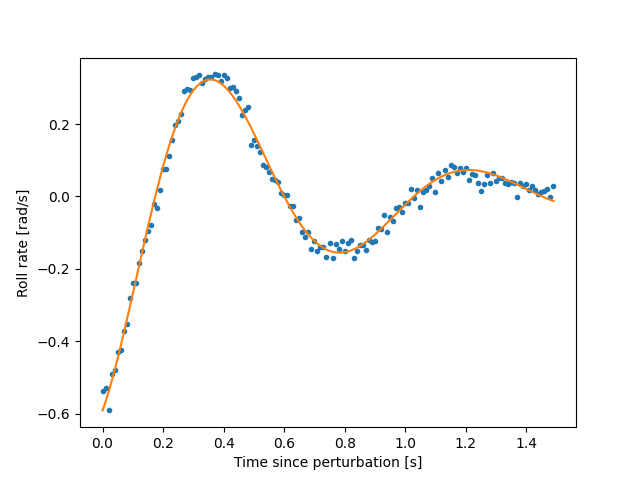
\includegraphics[width=\columnwidth]{figures/example_roll_rate_fit.png}
    \caption{Example of a fit of a decaying oscillation to roll rate data.} \label{example-roll-rate-fit}
\end{figure}

\section{Results}
The mean, minimal and maximal $r^2$ value for the fitted function on the roll data can be seen in
table \ref{table-r-squared.} A plot of the measured eigenvalues for different gains of the
balance-assist controller can be seen in figure \ref{fig-all-gains}. Furthermore, the measured
eigenvalues for gain -6 can be seen in table \ref{table-eigenvalues-gain-6}, for gain -8 in table
\ref{table-eigenvalues-gain-8} and for gain -10 in table \ref{table-eigenvalues-gain-10}.

\begin{figure}
    \centering
    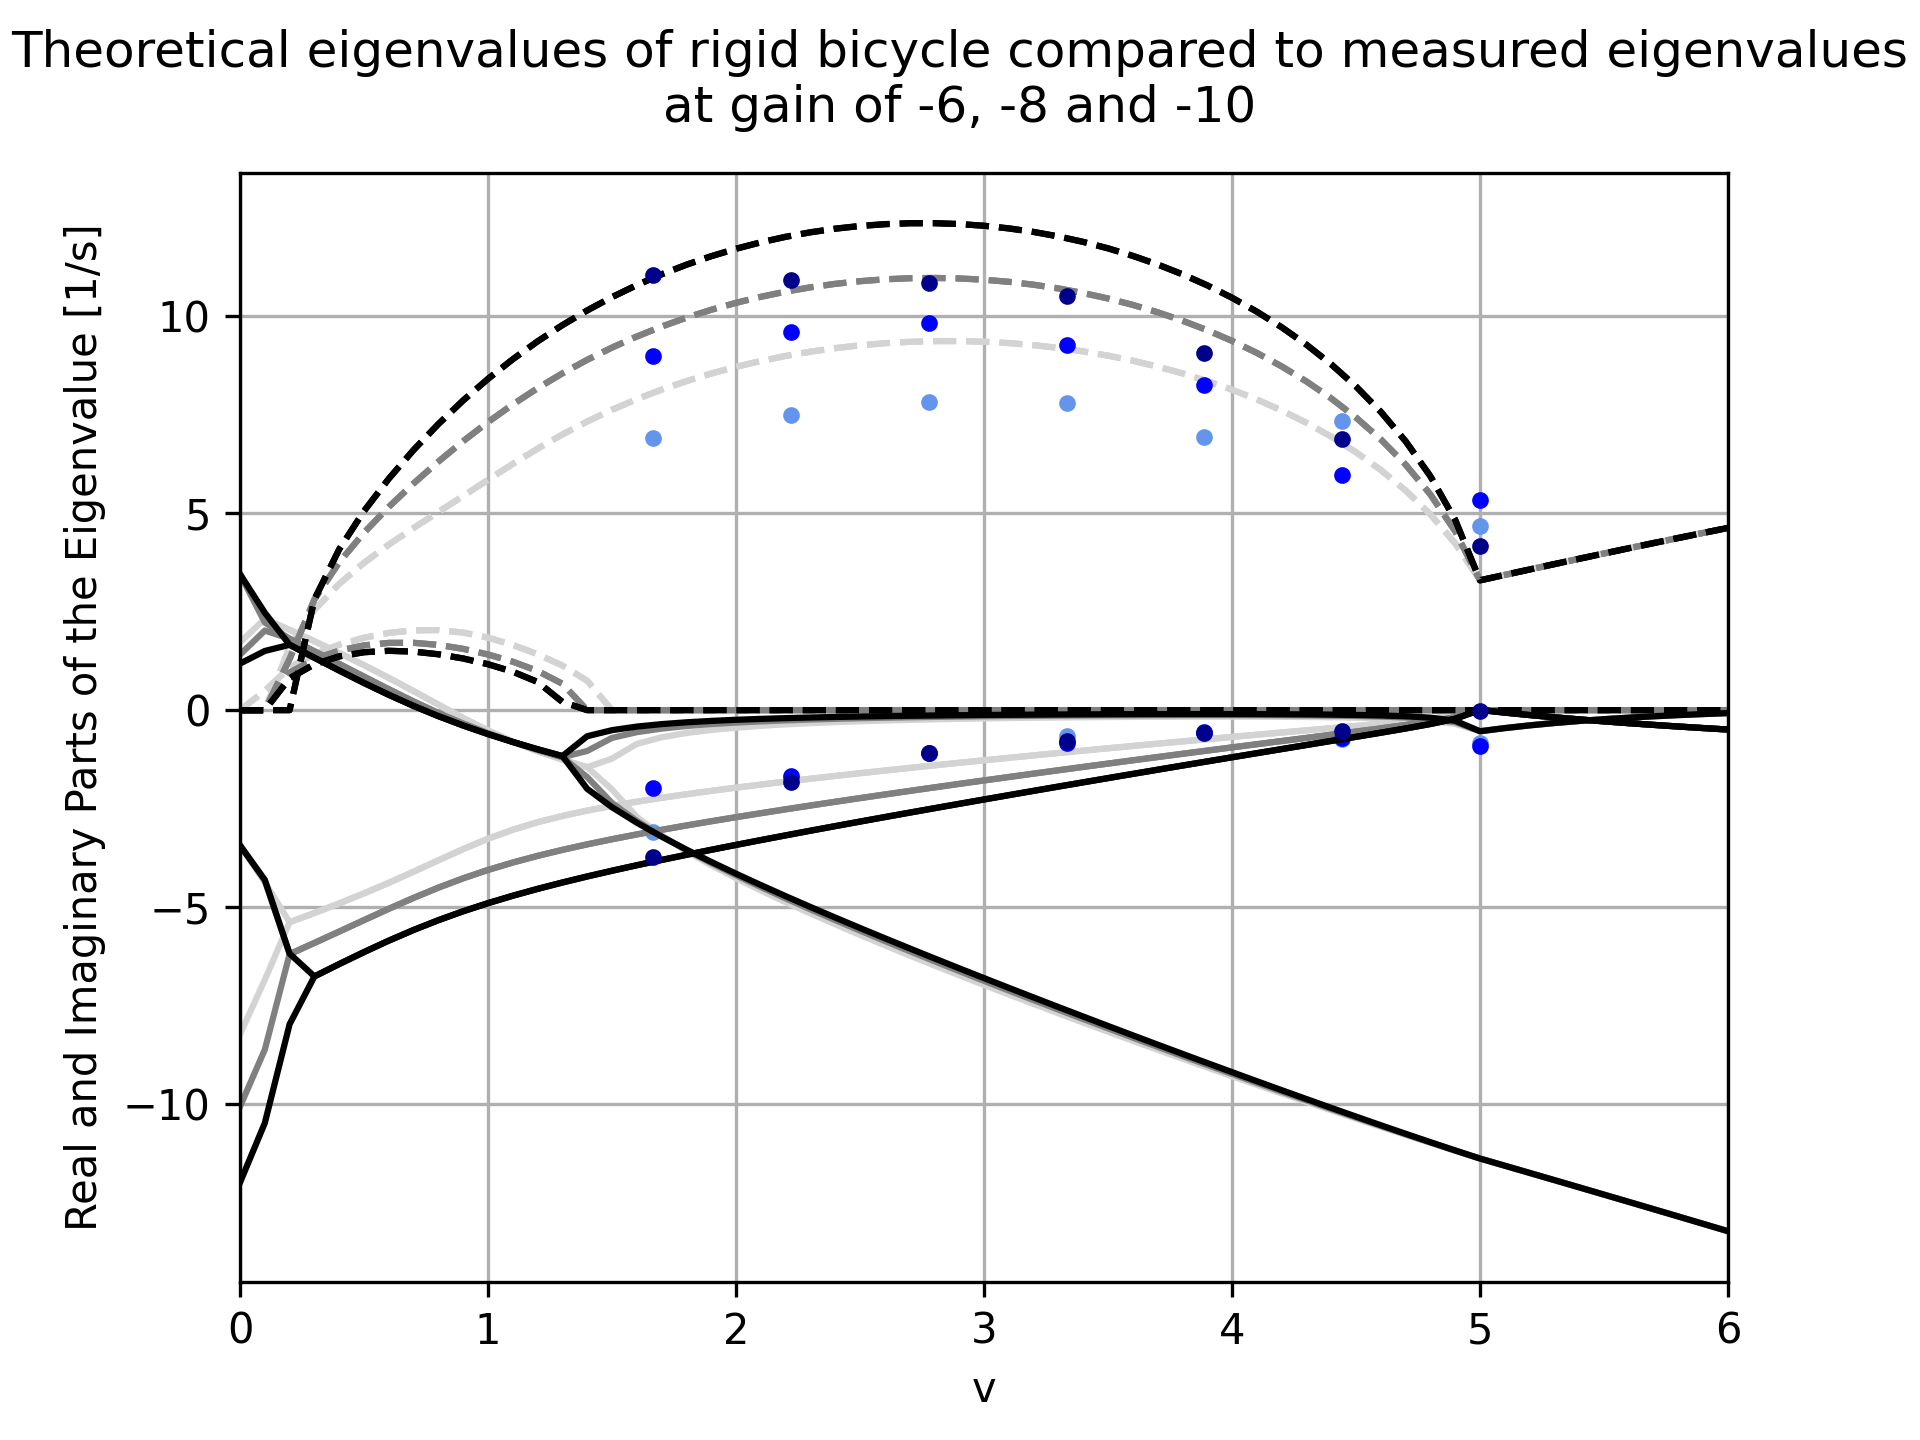
\includegraphics[width=\columnwidth]{figures/all-gains.png}
    \caption{Theoretical eigenvalues of the rigid bicycle with added balance-assist and control compared to the
        measured eigenvalues of the balance-assist bicycle. The lightest color represents a gain of -6, the
        medium color a gain of -8 and the dark color a gain of -10.} \label{fig-all-gains}
\end{figure}

\begin{table}[]
    \centering
    \caption{Mean, maximal and minimal $r^2$ for the three gains.} \label{table-r-squared}
    \begin{tabular}{c|c|c|c}
        \textbf{Gain} & \textbf{Mean} & \textbf{Minimal} & \textbf{Maximal} \\ \hline
        -6            & 0.98          & 0.81             & 1.00             \\
        -8            & 0.99          & 0.98             & 1.00             \\
        -10           & 0.97          & 0.82             & 0.99
    \end{tabular}
\end{table}

\begin{table}[]
    \centering
    \caption{Real and imaginary parts of the measured eigenvalues for a gain of -6.}
    \label{table-eigenvalues-gain-6}
    \begin{tabular}{c|c|c}
        \textbf{Velocity (m/s)} & \textbf{Real part} & \textbf{Imaginary part} \\ \hline
        1.66                    & -3.10437           & 6.90899                 \\
        2.22                    & -1.73230           & 7.47695                 \\
        2.78                    & -1.07677           & 7.81142                 \\
        3.33                    & -0.64501           & 7.79933                 \\
        3.89                    & -0.57419           & 6.93977                 \\
        4.44                    & -0.73719           & 7.33274                 \\
        5.00                    & -0.82591           & 4.65962
    \end{tabular}
\end{table}

\begin{table}[]
    \centering
    \caption{Real and imaginary parts of the measured eigenvalues for a gain of -8.}
    \label{table-eigenvalues-gain-8}
    \begin{tabular}{c|c|c}
        \textbf{Velocity (m/s)} & \textbf{Real part} & \textbf{Imaginary part} \\ \hline
        1.66                    & -1.96625           & 8.97518                 \\
        2.22                    & -1.67178           & 9.59152                 \\
        2.78                    & -1.08789           & 9.82538                 \\
        3.33                    & -0.82441           & 9.27701                 \\
        3.89                    & -0.56166           & 8.26214                 \\
        4.44                    & -0.70618           & 5.97152                 \\
        5.00                    & -0.90672           & 5.32524
    \end{tabular}
\end{table}

\begin{table}[]
    \centering
    \caption{Real and imaginary parts of the measured eigenvalues for a gain of -10.}
    \label{table-eigenvalues-gain-10}
    \begin{tabular}{c|c|c}
        \textbf{Velocity (m/s)} & \textbf{Real part} & \textbf{Imaginary part} \\ \hline
        1.66                    & -3.73303           & 11.03922                \\
        2.22                    & -1.83437           & 10.90979                \\
        2.78                    & -1.08183           & 10.84567                \\
        3.33                    & -0.78383           & 10.49930                \\
        3.89                    & -0.59061           & 9.07418                 \\
        4.44                    & -0.53405           & 6.87337                 \\
        5.00                    & -0.02263           & 4.16736
    \end{tabular}
\end{table}

\section{Discussion}
It is interesting that the weave mode is similarly damped for all three gains. In contrast, the
imaginary part of the eigenvalues increases as the gain gets larger. This would suggest that there
is no reason to set the gain any larger than -6.

Looking at the $r^2$ values in table \ref{table-r-squared}, it can be seen that the function in
equation \ref{kooijman-func} is fitted best to the roll data for a gain of -8. Both the -6 and -8
gains have a much lower minimal $r^2$. However, the average $r^2$ for these gains is still close to
1.

Future work can adjust the parameters of the bicycle model to better represent the measured
eigenvalues. For example, the \emph{symfit} package \cite{symfit} could be used to fit the symbolic
equations of motion of the bicycle model to the measured eigenvalues. Another approach would be to
optimize the gain of the theoretical controller to better approximate the measured eigenvalues. The
theoretical controller is not identical to the actual controller on the bicycle. By assuming the
parameters of the rigid bicycle approximately correct, the difference in the theoretical and
measured eigenvalues should be due to the difference in balance-assist controller.

\bibliographystyle{plain}
\bibliography{weave-experiments}

\end{document}